\section{Tests} % Tests
\begin{frame}
    \frametitle{Tests}
    \pause
    \begin{block}{Elektronik}
        \begin{itemize}
            \item Sensoren zur Korberkennung
            \item BLDC Treiber
        \end{itemize}
    \end{block}
    \pause
    \begin{block}{Mechanik}
        \begin{itemize}
            \item Schussvorrichtung
            \item Drehvorrichtung
        \end{itemize}
    \end{block}
    \pause
    \begin{block}{Informatik}
        \begin{itemize}
            \item Bilderkennung
        \end{itemize}
    \end{block}
\end{frame}

\subsection{Elektronik}
\begin{frame}
    \frametitle{Sensoren}
    \begin{columns}
        \pause
        \begin{column}{0.5\textwidth}
            \begin{block}{Ultraschall - HC-SR04}
                \begin{itemize}
                    \item Laufzeit Ultraschallimpuls
                    \item $D = \frac{T \cdot c_{Luft}}{2}$
                \end{itemize}
                \pause
                \begin{figure}
                    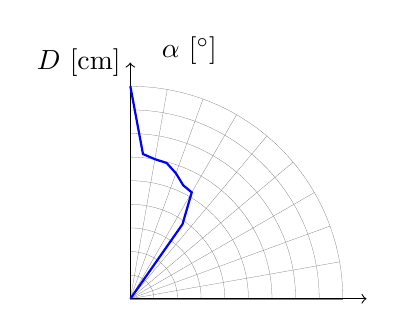
\begin{tikzpicture}[scale=1.5]
                        % Grid
                        % Grid for Angle
                        \foreach \i in {0, 10, ..., 90}
                        {
                            \draw[ultra thin, gray]
                                (90-\i:0) -- (90-\i:1.8);
                                %node[above right, black] {\i};
                        }
                        % Grid for Distance
                        \foreach \i in {0, 20, ..., 180}
                        {
                            \draw[ultra thin, gray]
                                (0.01*\i,0) arc [radius = 0.01*\i, start angle = 0, end angle = 90];
                                %node[left, black] {\i};
                        }
                        % Axis
                        \draw[->] (0:0) -- (0:2);
                        \draw[->] (0:0) -- (90:2) node[left] {$D$ [cm]};
                        \node at (0.5, 2.1) {$\alpha$ [$^\circ$]};
                        % Data
                        \draw[thick, blue]
                            (90 - 0  : 1.80) --
                            (90 - 5  : 1.23) --
                            (90 - 10 : 1.20) --
                            (90 - 15 : 1.19) --
                            (90 - 20 : 1.13) --
                            (90 - 25 : 1.06) --
                            (90 - 30 : 1.04) --
                            (90 - 35 : 0.77) --
                            (90 - 40 : 0.00) ;
                    \end{tikzpicture}
                \end{figure}
            \end{block}
        \end{column}
        \pause
        \begin{column}{0.5\textwidth}
            \begin{block}{Infrarot - GP2Y0A710K0F}
                \begin{itemize}
                    \item Triangulation
                    \item $D = d \cdot \arctan(\alpha)$
                \end{itemize}
                \pause
                \begin{figure}
                    \includegraphics[width=0.8\textwidth]{../doc/fig/scope_80.png}
                \end{figure}
            \end{block}
        \end{column}
    \end{columns}
\end{frame}

\begin{frame}
    \frametitle{BLDC}
\end{frame}

\subsection{Mechanik}
\begin{frame}
    \frametitle{Schussvorrichtung}
\end{frame}
\begin{frame}
    \frametitle{Drehvorrichtung}
\end{frame}

\subsection{Informatik}
\begin{frame}
    \frametitle{Bildverarbeitung}
\end{frame}

